\documentclass{article}
\usepackage{amsmath, amssymb}
\usepackage{cancel}
\usepackage{tikz}
\usepackage{tikz-cd}
\usepackage{mdframed}
\usepackage{hyperref}
\usetikzlibrary{automata, positioning, arrows}

\begin{document}

\section{Lecture 16: Plan for Class}
Last time:
\begin{enumerate}
    \item Chaos in 1-D maps \[ x\mapsto 2x \pmod 1 \]
    \item Period-3 implies chaos (Li-Yorke)
    \item Sharkovskii's theorem (Theorem 6.3.11 in GH)
\end{enumerate}

Today:
\begin{enumerate}
    \item Cantor-sets and dynamics on them 
    \item Smale horseshoe \S 5.1
    \item Hyberbolic structure \S 5.2
    \item Markov partitions \S 5.2
    \item Smale-Birkhoff theorem \S 5.3
\end{enumerate}
Rowley said we probably won't get time for `Hyberbolic structure' and `Markov partitions'.

\section{Cantor sets and dynamics on them}

\subsection{Cantor set}

This is a fairly standard topic in an introductory real analysis course, but for completeness, we have the following sets 

\begin{table}[h!]
    \centering
    \begin{tabular}{|c|c|c|}
    \hline
    Label & Construction & Length \\
    \hline
    $I_0$ & $[0,1]$ & 1 \\
    $\Lambda_1$ & $[0,\frac{1}{3}]\bigcup [\frac{2}{3},1]$ & $2\times\frac{1}{3}=\frac{2}{3}$ \\
    $\Lambda_2$ & $[0,\frac{1}{9}]\bigcup [\frac{2}{9},\frac{1}{3}] \bigcup [\frac{2}{3},\frac{7}{9}]\bigcup [\frac{8}{9},1]$ & $\frac{4}{9}$ \\
    $\Lambda_k$ & $\cdots$ & $2^k \cdot \frac{1}{3^k}=\left(\frac{2}{3}\right)^k$\\
    \hline
    \end{tabular}
\end{table}

Let $k\to \infty$. What's left? Well, it's all the ``endpoints''. Whats the total ``length''? Well, it's $0$!
\[
\lim_{k\to \infty} \left(\frac{2}{3}\right)^k=0
\]
How about the \underline{cardinality}? That's a bit tricky, but doable!

Consider base-3 representations of points in $[0,1]$.
\[
0.211021001 = 0.a_1a_2a_3=a_1\cdot\frac{1}{3} + a_2\cdot\frac{1}{9} + a_3\cdot\frac{1}{27} + \cdots = \sum_{k=1}^{\infty}a_k\cdot\left(\frac{1}{3^k}\right)
\]
Now we can reason about our new representation at each step of the cantor set construction 
\begin{enumerate}
    \item @ step 1, eliminate numbers with a $1$ in first slot
    \item @ step 2, eliminate numbers with a $1$ in second slot 
    \item $\vdots$
    \item @ step $k$, eliminate numbers with a $1$ in slot $k$
    \item $\vdots$
\end{enumerate}
At step $\infty$, we are left with all numbers with a base-3 expansion that do not have a $1$. But now, we can construct the following bijection:
\[
\text{pt in } [0, 1] \iff \text{pt in } \Lambda_\infty
\]

\[
\text{binary } \updownarrow \hspace{6cm} \updownarrow \text{ base 3}
\]

\[
0.10011000\ldots \longrightarrow 0.20022000\ldots
\]
Essentially, any number in the interval $[0,1]$ can be represented in a binary expansion, and then we can map it to points in $\Lambda_\infty$ by replacing all the 1's with 2's. Hence, $\Lambda_\infty$ is uncountable!

This example is nice because it shows that there can by uncountable sets with Lebesque measure zero.

\subsection{Dynamics on Cantor set}

We can think about a tripling map (as opposed to a doubling map) with the middle third deleted.

\vspace{1em}
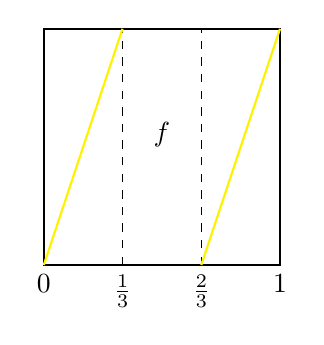
\begin{tikzpicture}[scale=3]
  % Axes box
  \draw[thick] (0,0) rectangle (1,1);

  % Dashed vertical lines at 1/3 and 2/3
  \draw[dashed] (1/3, 0) -- (1/3, 1);
  \draw[dashed] (2/3, 0) -- (2/3, 1);

  % Left branch: f maps [0, 1/3] -> [0, 1]
  \draw[thick, yellow] (0, 0) -- (1/3, 1);

  % Right branch: f maps [2/3, 1] -> [0, 1]
  \draw[thick, yellow] (2/3, 0) -- (1, 1);

  % x-axis labels
  \node[below] at (1/3, 0) {$\frac{1}{3}$};
  \node[below] at (2/3, 0) {$\frac{2}{3}$};
  \node[below] at (0,0) {$0$};
  \node[below] at (1,0) {$1$};

  % f label
  \node at (0.5, 0.55) {$f$};
\end{tikzpicture}

Consider pre-image of points in $I_0=[0,1]$ and other intervals on the Cantor set 
\begin{table}[h!]
    \centering
    \begin{tabular}{|c|c|}
    \hline
    Label & Construction \\
    \hline
    $I_0$ & $[0,1]$ \\
    $\Lambda_1 = f^{-1}\left(I_0\right)$ & $[0,\frac{1}{3}]\bigcup [\frac{2}{3},1]$  \\
    $\Lambda_2= f^{-1}\left(\Lambda_1\right) $ & $[0,\frac{1}{9}]\bigcup [\frac{2}{9},\frac{1}{3}] \bigcup [\frac{2}{3},\frac{7}{9}]\bigcup [\frac{8}{9},1]$\\
    $\Lambda_3 = f^{-1}\left(\Lambda_2\right)$ & $\cdots$ \\
    $\Lambda_k = f^{-1}\left( \Lambda_{k-1} \right)$ & $\cdots$ \\
    \hline
    \end{tabular}
\end{table}
The dynamics on this set are like the doubling map, where we perform the a shift operation, but instead on numbers with base-3 representation with no 1's.

Is there an invariant set in $[0,1]$? Yes! This is the Cantor set $\Lambda_\infty$\footnote{I'm actually not sure, I didn't follow this point}

\subsubsection{Upshot}

For this period tripling map, we get exactly the same ``symbolic dynamics'' as in the doubling map, but in a Cantor set (measure zero, But uncountable!)

\[
\Sigma = \{0,1\}^{\mathbb{Z}^+} \quad (0.10011000\ldots)
\]

\[
\sigma = \text{shift map}
\]
\[
\sigma: 0.a_1 a_2 a_3 \ldots \mapsto 0.a_2 a_3 a_4 \ldots
\]

\vspace{1em}

\begin{tikzcd}
\Lambda_\infty \arrow[r, "f"] \arrow[d] & \Lambda_\infty \arrow[d] \\
\Sigma \arrow[r, "\sigma"] & \Sigma
\end{tikzcd}

\subsection{Compare with $x\mapsto \mu x \left(1-x\right)$}

There is an uncountable invariant set $\Lambda$ on which dynamics are same as full ``shift on two symbols''.

\section{Smale's horseshoe}

To construct the Smale's horseshoe, first construct a map 
\[
[0,1]\times [0,1] \to \mathbb{R}^2
\]
where $[0,1]\times [0,1] =S$ and $S$ is the unit square.

Now squish the unit square horizontally, and then bend the top third around to come back into the unit square: this is the map $f$. Notice how the middle third is excluded from this new unit square. Essentially, each step of the construction of the Smale's horseshoe looks like a construction of the Cantor set.

Performing this infinitely many times, we get $\Lambda_+$, an invariant set applying $f$ consisting of vertical strips on $S$.

\subsection{Inverse map}

Just like how we constructed Smale's horseshoe, we can do it in reverse, by squishing vertically instead of horizontally: this is the map $f^{-1}$.

Performing $f^{-1}$ infinitely many times, we get $\Lambda_-$, an invariant set applying $f^{-1}$ consisting of horizontal strips on $S$.

\subsection{Forward and inverse map}

We can define $\Lambda$, an invariant set, via the intersection of $\Lambda_+$ (vertical strips) and $\Lambda_-$ (horizontal strips). We can then index points on $\Lambda$ by which vertical strip they lie in at each iterate. To each $x\in\Lambda$, associate a bi-infinite sequence $\{0,1\}^{\mathbb{Z}}$ by writing 
\[
\varphi(x) = (a_j)^\infty_{j=-\infty} \quad \text{with} \quad \begin{cases}
    0 \text{ if } f^j\in H_0 \\
    1 \text{ if } f^j\in H_1
\end{cases}
\]

\subsection{Need a metric}

We need a metric on $\sum = \left\{0,1\right\}^{\mathbb{Z}}$. Say we have two sequences 
\[
a=(a_j)\in\sum, \qquad b=(b_j)\in\sum
\]
then we can define a metric 
\[
d(a,b) = \sum_{j=-\infty}^{\infty}\frac{\left| a_j - b_j \right|}{2^{\left| j \right|}}
\]
where sequences are close if they agree on a long central stretch of values.

\subsection{A theorem}

\underline{Theorem 5.1.1} $f\big|_\Lambda$ is homeomorphic to shift map $\sigma$

This theorem, in conjunction with our metric, means that two sequences can agree on a long stretch of values, but then eventually, that long stretch of values will be shifted out, and the values not agreed on dominate. This means there is a sensitivity on initial conditions.

\section{Smale-Birkhoff theorem \S 5.3}

This theorem, theorem 5.3.5 in the book, will imply that ``transverse homoclinic points imply horseshoes''.

\underline{Theorem}: Let $f:\, \mathbb{R}^n\to \mathbb{R}^n$ have a hyperbolic fixed point $p$ with a transverse homoclinic point $q$. Then $f$ has a hyperbolic invariant set $\Lambda$ such that $f\big|_\Lambda$ is homeomorphic to a shift $\sigma$.



\end{document}